\documentclass[11pt]{article}
\usepackage[margin=1in]{geometry}
\usepackage{amsmath,amssymb,graphicx,booktabs,microtype,xcolor}
\usepackage[numbers,sort&compress]{natbib}
\usepackage{caption,float}
\usepackage[hidelinks]{hyperref}
\captionsetup{font=small,labelfont=bf}
\hypersetup{pdftitle={Choosing a Vision Tower for a Text-Only LLM},pdfauthor={Immanuel Peter}}
\setlength{\emergencystretch}{1em}
\title{Choosing a Vision Tower for a Text-Only LLM\\
\large A frozen-representation study of six vision towers}
\author{Immanuel Peter\\University of Chicago\\\texttt{ipeter@uchicago.edu}}
\date{September 2026}
\begin{document}
\maketitle
\begin{abstract}
Vision encoders with similar recognition accuracy can support different spatial tasks.
We compare six frozen vision towers across recognition, depth, surface normals,
correspondence, and occlusion, and examine internal layers and native multimodal
connectors. Three patterns emerge. Capability profiles differ across towers and label
budgets; the two highest full-label recognition estimates are statistically unresolved.
Geometry peaks before the final layer in 23 of 24 task--tower--capacity combinations,
while recognition peaks at the final layer in 19 of 24 tower--readout--capacity combinations. Finally, projected
features improve probe performance over final tower features in all 16 DIODE geometry
comparisons, with 15 paired intervals excluding zero. This pattern does not extend to
KITTI, where two comparisons reverse and two are unresolved, or uniformly across
correspondence datasets. These are measurements of recoverability under specified
readouts, not information content or downstream language-model performance. A lossless
merge changes correspondence scores substantially, illustrating that distinction.
We document the unresolved recognition-pooling control, native-grid confound, and
protocol corrections alongside the results.
\end{abstract}
\section{Introduction}
Adding vision to a language model requires choosing an encoder, an extraction layer,
and a connector. A full vision-language model (VLM) evaluation measures their combined
behavior after training. Frozen-feature probes answer a narrower question: what can a
specified readout recover at each point in the visual pipeline? This can identify
candidate representations before multimodal training, although their usefulness to a
language model must still be tested downstream.

We study DINOv2 \citep{oquab2024dinov2} and SigLIP2 \citep{tschannen2025siglip2} as
standalone references, alongside towers extracted from Kimi K2.6 \citep{moonshot2026kimik26},
Kimi K3 \citep{moonshot2026kimik3}, Muse Glimmer \citep{meta2026museglimmer}, and
Qwen3.8 \citep{qwen2026qwen38}. Recognition asks which category an image
contains. Geometry asks how far surfaces are from the camera and which direction they
face. Correspondence asks whether features match the same point across views or related
parts across objects. Occlusion tests recognition as visible image content is removed.
These capabilities need not favor the same representation.

The benchmark resolves internal layers and, for multimodal towers, the native merge and
projector stages. Towers and connectors remain frozen; recognition and geometry use
trained readouts, while correspondence uses direct feature matching. The study contributes
capability profiles for six towers, layer sweeps under two readout-capacity settings, and
paired evidence that connector effects change across evaluation datasets. The accompanying
code and result records expose the measurements and the controls behind these claims.
We report effects under this protocol rather than proposing an overall tower ranking.

\section{Related work}
Prismatic VLMs and Cambrian-1 compare visual encoders through multimodal training and
complete VLM evaluations \citep{karamcheti2024prismatic,tong2024cambrian}.
Our study complements that approach by stopping at frozen visual features.
Probe3D provides the closest methodological foundation: frozen-feature probes for depth
and normals, and feature matching for correspondence \citep{elbanani2024probe3d}.
We adapt its dense readout to one extraction layer at a time and use DIODE for geometry.
These changes support layer comparisons but prevent interpreting our scores as a
reproduction of its published benchmark.

Intermediate features can outperform final features. Perception Encoder demonstrates
this across downstream tasks and introduces alignment methods to expose those features
at the output \citep{bolya2025perception}. We compare recognition and geometry along
normalized layer depth and follow the deepest features through native connectors.
Work beyond the encoder also motivates this stage analysis. Fu et al.
\citep{fu2025hidden} find visual information accessible inside VLMs that nevertheless
perform poorly on vision-centric tasks. Wu et al.\ \citep{wu2026dropoff} find a drop in
segmentation decodability at the adapter, followed by recovery in the language model.
These studies use different tasks and readouts; they do not establish a universal
preservation or loss rule. Our contribution is a joint comparison of towers, layers,
and connector stages under a shared protocol, with the limitations of probing made
explicit \citep{belinkov2022probing}.

\section{Benchmark design}
\label{sec:design}
\subsection{Towers and extraction points}
Table~\ref{tab:roster} lists the six towers. Each receives an image resized and
center-cropped to $448\times448$, with its native normalization and input packing.
At layer $i$ of a tower with $L$ blocks, relative depth is $i/L$. We sample
$i=\operatorname{round}(Lk/8)$ for $k=1,\ldots,8$; actual fractions vary slightly with $L$.
The deepest extraction includes final tower normalization where present; Qwen3.8
is read at the last block output, before normalization on the merger path.

\begin{table}[t]
\centering\small
\caption{Tower architectures. Tokens are measured before merging at $448\times448$.
The last column is the projector's output width. DINOv2 and SigLIP2 have no native
connector in this study.}
\label{tab:roster}
\begin{tabular}{lrrrrr}
\toprule
Tower & Layers & Width & Patch & Tokens & Projected width\\
\midrule
DINOv2-L & 24 & 1024 & 14 & 1024 & ---\\
SigLIP2-so400m & 27 & 1152 & 14 & 1024 & ---\\
Kimi K2.6 & 27 & 1152 & 14 & 1024 & 7168\\
Kimi K3 & 27 & 1024 & 14 & 1024 & 7168\\
Muse Glimmer & 50 & 1536 & 14 & 1024 & 6656\\
Qwen3.8 & 27 & 1152 & 16 & 784 & 5120\\
\bottomrule
\end{tabular}
\end{table}

For each multimodal tower, we also extract \texttt{merged}, which concatenates each
$2\times2$ group of patch tokens, and \texttt{projected}, the learned map into the
parent language model's embedding width. These stages exist only after the final tower
layer. We do not apply projectors to intermediate layers or exchange them between towers.
Thus the experiment separates extraction points within native pipelines, rather than
independently crossing every tower, layer, and projector.

\subsection{Tasks and readouts}
Recognition uses the 13,000-image validation export of \texttt{ilee0022/ImageNet100},
a 100-class ImageNet subset \citep{deng2009imagenet,ilee0022imagenet100}, split by us into
9,100 training, 1,950 validation, and 1,950 test images. A linear classifier reads either
the mean feature or a learned attention pool. Both operate on a cached $4\times4$ pooled
grid. We report top-1 accuracy after 20 training epochs. Label-budget runs keep validation
and test fixed and train on 100, 455, 1,820, or 9,100 images. The nominal 1\% condition
uses one image per class, hence 1.10\% of the training split.

Geometry uses DIODE depth and normals \citep{vasiljevic2019diode}, with 541 training,
115 validation, and 115 test images drawn from its validation release. The test split
contains 51 indoor and 64 outdoor images. A Probe3D-style multiscale decoder reads the
full patch grid from one layer and trains for 10 epochs. Depth is summarized by
$\delta_1$, the mean per-image fraction of valid pixels satisfying
$\max(\hat d/d,d/\hat d)<1.25$, for prediction $\hat d$ and target $d$; higher is better. Normals use mean angular error in
degrees; lower is better. Targets cover the same crop as the input image.

Correspondence uses cosine feature matching on NAVI, ScanNet, and SPair-71k
\citep{jampani2023navi,dai2017scannet,min2019spair}. NAVI measures recall within 2\,cm
across views of an object; ScanNet measures recall within 10 pixels across indoor views;
SPair measures keypoint accuracy within 10\% of the target bounding-box scale across
object instances. NAVI and ScanNet match on a $64\times64$ feature grid; SPair matches
annotated keypoints against each stage's own grid. These metrics are not averaged together. Occlusion measures top-1 accuracy after masking
0, 10, 20, 35, or 50\% of image area, with readouts trained once on clean images.

KITTI provides a separate depth experiment with 700 training, 150 validation, and
150 test images \citep{geiger2012kitti,uhrig2017sparsity}. We retrain the depth readout
on KITTI to test whether the DIODE stage ordering recurs. This is not zero-shot transfer
of a DIODE-trained readout. Dataset preparation and evaluation details appear in
Appendix~\ref{app:protocol}.

\subsection{Capacity, selection, and uncertainty}
\label{sec:selection}
The core recognition and DIODE sweeps run at native feature width (\emph{raw}) and after
training-split PCA to 512 dimensions (\emph{matched}). PCA is frozen before readout training. Matching
holds head parameter count constant within a readout type; it does not equate spatial
sampling or the information retained by the reduction. We retain both arms as a
sensitivity analysis.

A cell specifies tower, extraction point, task/readout, and capacity arm. The core sweeps
contain 224 recognition and 224 geometry cells. Each selects its learning rate on
validation from a shared task-specific grid, then trains with three seeds. Headline
intervals use 10,000 paired bootstrap resamples at 95\% confidence. For trained readouts,
we first average each image's score over seeds, then resample images; correspondence
resamples image pairs. These intervals condition on the fitted runs and do not include
all training uncertainty. We report seed standard deviations separately. Intervals are
pointwise, without a multiple-comparison correction. An interval crossing zero is
unresolved, not evidence of equivalence; an untested pair has no inferential ranking.

\subsection{Controls and corrections}
\label{sec:controls}
Extraction tests compare weights with parent checkpoints and restore spatial token order
before dense evaluation. Kimi K3 has tower-weight equality but lacks the forward-output
and projector-weight checks available for the other extracted models. Lossless merging
is verified against cached tensors for the two Kimi towers and inferred from architecture
for Muse Glimmer and Qwen3.8.

The pooled recognition cache has an incomplete control. On SigLIP2 and Muse Glimmer,
mean-readout results agree with full-token features, but six of sixteen full-token
attention cells collapse during optimization. Follow-up runs do not establish stable
agreement. Attention-based recognition levels and layer curves therefore remain
conditional on pooled features.

Two corrections changed the recorded results: expanding the recognition learning-rate
grid and seeding randomized PCA. Initially, 107 of 224 cells selected the lower rate
limit. In the corrected run none selects the lower limit and three select the upper
limit. All matched recognition cells and headline geometry comparisons were rerun. Together these corrections changed an apparent Muse
Glimmer merge-to-projector loss from $-0.0075$ to $+0.0042$ top-1. The full matched geometry sweep retains its original
randomized reductions. Its curves and selected peaks are descriptive; geometry intervals
refer to deterministic reruns. Appendix~\ref{app:corrections} records the corrections.

\section{Results}
\subsection{Capabilities and label budgets favor different towers}
\label{sec:profiles}
Table~\ref{tab:capability} shows capability profiles without an aggregate score.
DINOv2 has the highest measured depth, normal, and NAVI performance, while Muse Glimmer
has the highest full-label recognition estimate and the lowest tower-stage scores on
all three correspondence datasets. These are observed levels; most cross-tower pairs
have not been tested with intervals.

\begin{table}[t]
\centering\small
\caption{Capability profiles. Recognition uses the label-budget runs at 1\% and 100\%,
with final-layer features and the matched attention readout. Depth and normals are the best observed matched test scores across sampled
layers, not independently validated layer selections. NAVI uses the final layer.
Retention is accuracy at 50\% occlusion divided by clean accuracy. Higher is better except
for normals. No overall rank is assigned.}
\label{tab:capability}
\begin{tabular}{lrrrrrr}
\toprule
Tower & 1\% labels & Full labels & Depth $\uparrow$ & Normals $\downarrow$ & NAVI $\uparrow$ & Retention\\
\midrule
DINOv2 & 0.3689 & 0.9079 & 0.7015 & 18.85 & 0.5389 & 0.5194\\
SigLIP2 & 0.6559 & 0.9168 & 0.6702 & 23.90 & 0.4013 & 0.4883\\
Muse Glimmer & 0.4330 & 0.9212 & 0.6588 & 24.30 & 0.2139 & 0.5163\\
Kimi K2.6 & 0.3448 & 0.8862 & 0.6595 & 25.51 & 0.3646 & 0.2786\\
Qwen3.8 & 0.2451 & 0.8791 & 0.6736 & 24.24 & 0.3785 & 0.3046\\
Kimi K3 & 0.2191 & 0.8369 & 0.6546 & 27.03 & 0.3334 & 0.2042\\
\bottomrule
\end{tabular}

\end{table}

Three full-label recognition comparisons have paired intervals in the matched attention
arm. Muse Glimmer exceeds DINOv2 by $0.0125$ $[0.0034,0.0215]$ top-1. Muse Glimmer versus
SigLIP2, $0.0041$ $[-0.0036,0.0121]$, and SigLIP2 versus DINOv2,
$0.0084$ $[-0.0009,0.0178]$, remain unresolved. The data therefore do not establish a
unique full-label recognition winner.

The label budget changes the observed ordering (Figure~\ref{fig:labels}). With one
training image per class, SigLIP2 reaches 0.6559 top-1, compared with Muse Glimmer's
0.4330. At full labels their estimates converge to 0.9168 and 0.9212. Qwen3.8's nominal
1\% cell is unstable: its seed standard deviation is 0.0780 around a mean of 0.2451.
These curves describe label efficiency under the pooled attention readout, whose
full-token control remains inconclusive.

\begin{figure}[t]
\centering
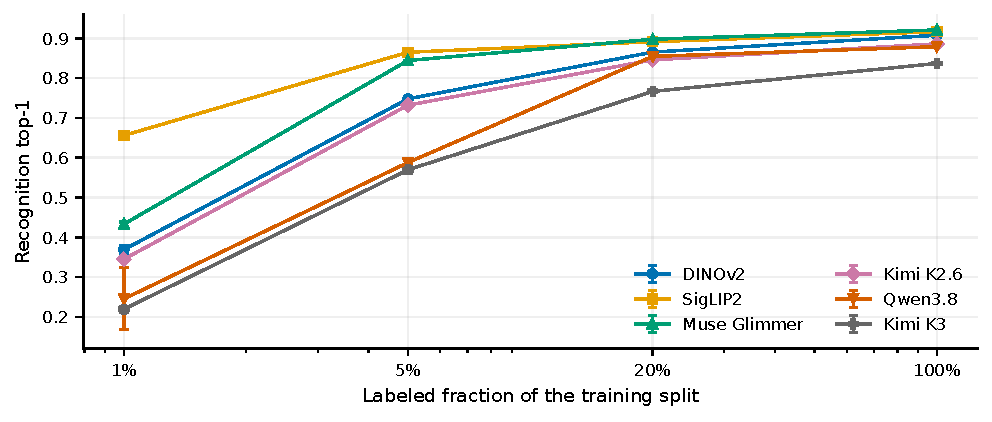
\includegraphics[width=\textwidth]{figures/paper-label-budget.pdf}
\caption{Recognition across label budgets at the final tower layer, matched attention arm.
Points average three seeds; vertical bars show one seed standard deviation, not confidence
intervals. The nominal 1\% budget contains 100 images.}
\label{fig:labels}
\end{figure}

Two cross-tower geometry comparisons were rerun with deterministic PCA at layers
selected from the test-score sweep, without independent validation of that selection. DINOv2 exceeds
Qwen3.8 in depth by $0.0292$ $[0.0099,0.0484]$ $\delta_1$, but that comparison also
changes native grid size from $28\times28$ to $32\times32$. DINOv2 reduces normal error
relative to SigLIP2 by $5.0370$ $[4.3038,5.8164]$ degrees; both use $32\times32$ grids.
These intervals support the named comparisons under their protocols, not a complete
geometry ranking.

Occlusion adds another distinction. At 50\% masking, DINOv2, Muse Glimmer, and SigLIP2
retain approximately half their clean accuracy, compared with 20--31\% for the other
three towers. This grouping is descriptive: available occlusion intervals compare clean
and perturbed images within a stage, not retention between towers.
Appendix~\ref{app:secondary} gives the curves and stage-level interpretation.

\subsection{Geometry usually peaks before the final layer}
\label{sec:layers}
Across two capacity arms, geometry has a pre-final test-score peak in 23 of 24
combinations of tower, task, and capacity arm. The exception is DINOv2 depth in the raw arm.
Recognition reaches its highest score at the final layer in 19 of 24 combinations of
tower, readout, and arm. Figure~\ref{fig:layers} shows attention recognition, depth, and
normals for both arms; Appendix~\ref{app:peaks} lists the geometry peaks.

In the matched arm, choosing the final layer instead of the best observed layer reduces
depth $\delta_1$ by 0.0256--0.1422 and increases normal error by 4.34--10.22 degrees.
These are descriptive sweep differences: the peak was identified on the same test
scores being compared, and intervals were not computed for every peak-to-final contrast.
The result motivates validating intermediate layers for spatial tasks. It does not
establish a universal optimal fraction of tower depth.

\begin{figure}[t]
\centering
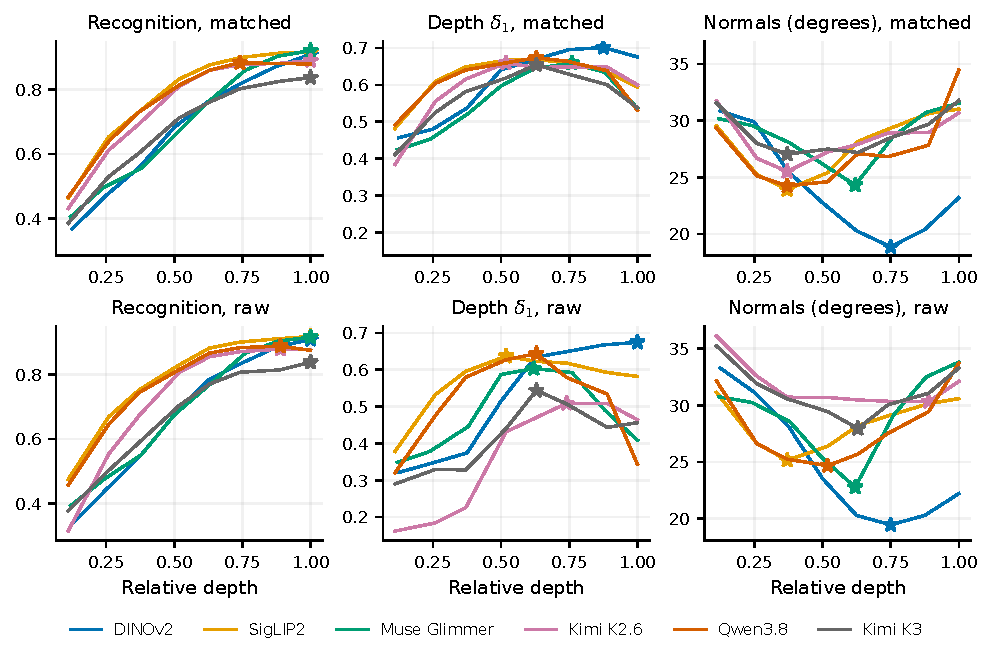
\includegraphics[width=\textwidth]{figures/paper-layers.pdf}
\caption{Layer sweeps at the tower stage. Columns show recognition with attention pooling,
DIODE depth, and DIODE normals; rows show matched and raw arms. Stars mark each curve's
best observed test score. Recognition uses pooled tokens; geometry uses full patch grids.
Matched geometry curves come from the original randomized-PCA sweep.}
\label{fig:layers}
\end{figure}

Qwen3.8 accounts for four recognition curves whose peak is earlier than the final layer;
Kimi K2.6 raw attention accounts for the fifth. Qwen3.8's earlier-layer advantage resolves
in raw attention, $0.0128$ $[0.0053,0.0203]$, and raw mean,
$0.0156$ $[0.0053,0.0263]$. Its two matched comparisons cross zero. The nominal Kimi
K2.6 decline is smaller than its seed standard deviation and was not tested with an
interval. Thus even this exception depends on the readout and capacity setting.

\subsection{Connector effects change across evaluations}
\label{sec:projectors}
We expected the connector to reduce spatial recoverability. DIODE gives the opposite
pattern: all 16 projected-versus-final-tower comparisons favor projected features, and
15 paired intervals exclude zero. These comprise four connectors, two geometry tasks,
and two capacity arms. The unresolved comparison is Kimi K2.6 raw depth,
$0.0196$ $[-0.0003,0.0402]$ $\delta_1$.

\begin{figure}[t]
\centering
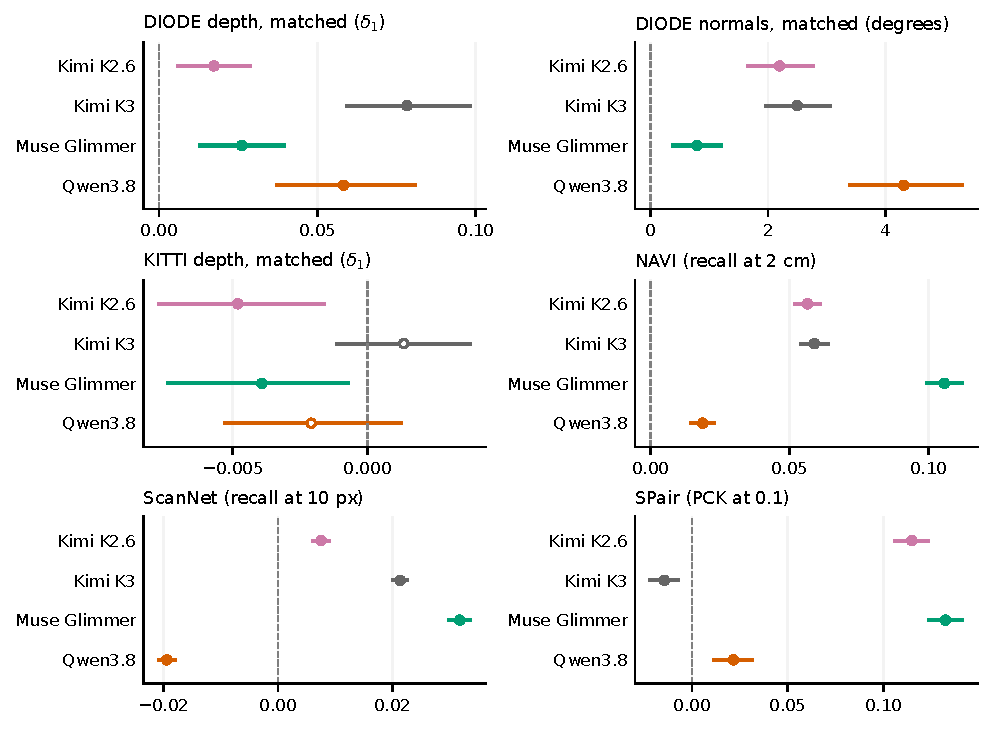
\includegraphics[width=\textwidth]{figures/paper-projectors.pdf}
\caption{Projected features versus final tower features. Positive favors projected;
for normals the difference is tower error minus projected error. DIODE and KITTI panels
use matched readouts; correspondence is training-free. Bars are paired 95\% intervals,
with open markers where they cross zero. Each panel has its own metric and scale.
Appendix~\ref{app:intervals} includes both geometry arms and exact values.}
\label{fig:projectors}
\end{figure}

The matched DIODE gains range from 0.0174 to 0.0784 in depth $\delta_1$ and from
0.7924 to 4.3130 degrees of normal-error reduction. The largest raw depth gain is
Qwen3.8's 0.1601, compared with 0.0584 after capacity matching. Because PCA also changes
the input representation, the difference between arms is a sensitivity result rather
than an isolated estimate of the effect of head size.

On KITTI, Kimi K2.6 and Muse Glimmer reverse: projected-minus-tower differences are
$-0.0048$ $[-0.0077,-0.0016]$ and $-0.0039$ $[-0.0074,-0.0007]$ $\delta_1$, respectively.
Kimi K3 and Qwen3.8 are unresolved. Training new readouts on driving scenes therefore
does not reproduce the uniformly positive DIODE pattern. The datasets differ in scene
content, target coverage, depth range, and sample size; this study does not isolate
which difference causes the reversal.

Correspondence yields ten positive and two negative intervals, all excluding zero.
Qwen3.8's projected-minus-tower difference is $+0.0188$ $[0.0146,0.0230]$ on NAVI but
$-0.0194$ $[-0.0208,-0.0180]$ on ScanNet. Kimi K3's SPair difference is
$-0.0144$ $[-0.0216,-0.0070]$, while both geometric correspondence differences are positive. SPair compares
parts across different object instances, so this result concerns a different capability
from NAVI's same-object multiview consistency.

\subsection{Lossless merging exposes readout sensitivity}
\label{sec:merge}
A stage score can change even when the transformation discards no information.
On NAVI, Qwen3.8 scores 0.3785 at the tower stage, 0.1130 after merging, and 0.3973 after
projection. Merging concatenates neighboring tokens; it changes the vectors compared by
cosine matching and their spatial sampling. The drop therefore cannot by itself establish
information loss. Kimi K2.6 and Muse Glimmer show the same drop-and-recovery pattern.

This control demonstrates sensitivity to representation format. It does not provide a
numerical bound on the portion of a projector effect attributable to that sensitivity.
Likewise, a trained depth probe can recover more from projected features without the
projector adding new image information. Throughout, the measured outcome is performance
under a particular readout and training procedure.

\section{Implications for tower selection}
The practical use of these results is to narrow candidates and extraction points for a
specified task. SigLIP2 has the highest low-label recognition point estimate; DINOv2
has the highest geometry and NAVI estimates, often at intermediate layers for geometry.
These descriptive patterns suggest candidates for validation, not an inferential ranking.
At full labels, the Muse Glimmer--SigLIP2 recognition difference is unresolved, and the
native-grid difference limits the interpretation of DINOv2 versus Qwen3.8 depth.

Tower and layer should be evaluated together. Their optima differ by task, and an
intermediate feature may be poorly matched to a projector trained on final-layer output.
We have not tested reconnecting those layers to a language model. Nor do DIODE gains
justify selecting a connector for another domain: KITTI and correspondence show that
its measured effect can change sign. A deployment decision still requires the intended
readout, data distribution, and downstream training recipe.

\section{Limitations}
\label{sec:limitations}
The attention recognition results depend on $4\times4$ pooling whose full-token control
is inconclusive. This affects both cross-tower comparisons and layer-curve shape;
sharing a pooling operation does not guarantee it distorts all layers equally.
Mean-readout agreement was established on two towers, not the entire roster.
Geometry always uses full patch tokens.

DIODE and KITTI have only 115 and 150 test images, and DIODE readouts train on just
541 images. Equal training-set size does not imply equal underfitting across models.
Bootstrap intervals resample images or pairs, not independent scenes, objects, or new
training runs; correlations among units may make them overconfident. The selected
headline comparisons are not a family-wide significance test. Layer peaks selected
from test scores are descriptive and require separate validation before operational use.

PCA controls head width but can affect representations differently, and the full matched
geometry matrix has not been rerun with deterministic PCA. Qwen3.8's $28\times28$
native grid differs from the other towers' $32\times32$ grids. A common-grid sensitivity
experiment remains missing; neither PCA nor resizing correspondence maps establishes
identical original spatial information. Kimi K3 also lacks parent forward-output and
projector-weight parity checks, weakening confidence in its extracted pipeline.

Only rectangular occlusion was measured. The results do not establish robustness to blur,
scale, lighting, or other distribution shifts. Finally, frozen probing evaluates access
under our readouts. No language model is evaluated or adapted, and we do not test
whether the observed stage orderings survive multimodal training.

\section{Conclusion}
Vision-tower selection depends on the capability, label budget, and extraction point.
This six-tower study finds frequent intermediate-layer geometry peaks and consistent
DIODE probe gains after native connectors, alongside reversals on KITTI and two
correspondence comparisons. The useful next tests are domain-specific layer validation,
a stable full-token recognition control, common-grid geometry comparisons, and downstream
VLM evaluation of the selected representations.

\label{page:main-end}
\clearpage
\bibliographystyle{plainnat}
\bibliography{references}
\clearpage
\appendix
\section{Protocol and implementation details}
\label{app:protocol}
\subsection{Models and extraction}
The standalone references are DINOv2-L \citep{oquab2024dinov2} and
SigLIP2-so400m-patch14-384 \citep{tschannen2025siglip2}. The extracted pipelines come
from Kimi K2.6, Kimi K3, Muse Glimmer 30B, and Qwen3.8-27B
\citep{moonshot2026kimik26,moonshot2026kimik3,meta2026museglimmer,qwen2026qwen38}.
The repository adapters record their standalone checkpoint identifiers. The Qwen
result filenames retain the internal slug \texttt{qwen3\_5}; their recorded model ID
identifies the Qwen3.8 checkpoint evaluated here. Likewise, \texttt{moonvit\_v2}
identifies the Kimi K3 tower. Display names in this paper follow the recorded models.

At $448\times448$, patch-14 towers produce 1,024 tokens and Qwen3.8 produces 784.
Merging concatenates each $2\times2$ block, reducing these counts to 256 and 196 while
quadrupling feature width. The merged widths are 4,608 for Kimi K2.6 and Qwen3.8,
4,096 for Kimi K3, and 6,144 for Muse Glimmer. Native normalization and packing are
preserved; SigLIP2's position grid is interpolated from its configured resolution.
Qwen tower tokens are restored from merge-block order to raster order, and intermediate
Muse Glimmer tokens from attention-window order to raster order, before spatial scoring.

Extraction tests check exact parent weight equality for 335 packaged Kimi K2.6 tensors,
809 Muse Glimmer tensors, and 333 Qwen3.8 tensors, with parent stage-output comparisons.
Kimi K3 has equality checks for its 165 tower tensors. Its three exported projector
tensors are checked for compatible shapes, not equality to a separately loaded parent
projector; there is no parent forward-output comparison. These different validation
levels apply to every result that uses the respective adapter. Cache-level lossless-merge
checks cover Kimi K2.6 and Kimi K3; losslessness for the other two is inferred from the
implemented architecture.

\subsection{Datasets and spatial alignment}
ImageNet-100 uses the 13,000-image \texttt{validation} split of
\texttt{ilee0022/ImageNet100} \citep{ilee0022imagenet100}, exported by
\texttt{scripts/export\_imagenet100.py} and split with a fixed seed into
9,100/1,950/1,950 training/validation/test images. We identify the exact export because
ImageNet-100 does not designate a unique class list or split. The four label budgets subsample only
the training split and retain every class. Pooling to 16 tokens reduces recognition
cache storage; the full-token validation is described in Appendix~\ref{app:corrections}.

DIODE uses 771 validation-release images with normals, comprising 325 indoor and
446 outdoor images. The 541/115/115 split is fixed. Native $768\times1024$ images are
center-cropped consistently with the tower input; depth and normal targets retain their
native resolution within that crop. The observed depth range sets the head's bin ceiling
to 299.83\,m. A Probe3D-style multiscale decoder \citep{elbanani2024probe3d,ranftl2021dpt}
reads one layer, rather than combining four encoder layers. We train for 10 epochs with
AdamW \citep{loshchilov2019adamw}, batch size eight. The records also contain
$\delta_2$, $\delta_3$, RMSE, and scene-specific metrics. This single-layer, DIODE-based
protocol differs from the original Probe3D evaluation.

KITTI uses the selected-validation archive of the depth-completion dataset, partitioned
700/150/150. Readouts receive RGB features only; sparse depth provides targets.
Unsigned 16-bit depth is decoded in units of $1/256$\,m, zeros remain invalid, and
invalid pixels are masked in loss and evaluation. Mean valid coverage is 17.08\%, and
the recorded maximum depth is 85.766\,m. All towers use final tower features, with
projected features additionally evaluated for the four connectors, in the matched arm.

NAVI uses 555 wild-set pairs with relative rotations in $(0,120]$ degrees. ScanNet uses
1,500 pairs from the SuperGlue test split \citep{sarlin2020superglue}. SPair-71k samples
up to 200 pairs in each of 18 classes, for 3,600 pairs; the projected-versus-tower
intervals use 3,408 pairs with finite scores at both stages. NAVI and ScanNet features
are bicubically resized to $64\times64$ before cosine nearest-neighbor matching;
Lowe's ratio \citep{lowe2004distinctive} ranks up to 1,000 retained matches. ScanNet RGB
is aligned to the depth/intrinsics frame before cropping. SPair bilinearly samples
source features at annotated keypoints, then selects target grid centers by cosine argmax.
It uses each stage's own grid: $32\times32$ or $28\times28$ at the tower, and
$16\times16$ or $14\times14$ after merging/projection. It uses neither Lowe ranking nor
a top-1,000 cutoff. The SPair records' \texttt{evaluation\_side: 64} field is unused by
that scoring path. These protocols are adaptations of Probe3D. SPair aggregate levels are class-macro averages where labeled; bootstrap
contrasts average paired image-pair differences and use a different weighting.

Occlusion uses a fixed 2,000-image ImageNet-100 subset, with 300 held-out test images.
The reducer and attention readout are fitted on clean training features and frozen for
all masking conditions. Records include requested and actual occluded area, rectangle
coordinates, and fill value. Object scale and blur were planned but not measured.

\subsection{Readout capacity and learning rates}
Mean recognition averages tokens before a linear classifier. Attention recognition uses
a learned query, a 512-wide multihead projection, layer normalization, and a classifier.
The matched PCA arm fits the reduction on each cell's training features only, then
freezes it. Parameter counts after reduction are 51,300 for mean recognition,
1,627,748 for attention recognition, 1,444,608 for depth, and 1,314,819 for normals.
Raw heads grow with feature width. Matching parameter count does not ensure equal
optimization difficulty or equal representation distortion.

Recognition searches
$\{10^{-5},3\cdot10^{-5},10^{-4},3\cdot10^{-4},10^{-3},3\cdot10^{-3},
10^{-2},3\cdot10^{-2},10^{-1},3\cdot10^{-1},1\}$;
geometry searches
$\{10^{-4},3\cdot10^{-4},10^{-3},3\cdot10^{-3},10^{-2},3\cdot10^{-2}\}$.
The selected rate maximizes validation accuracy or depth $\delta_1$, or minimizes
validation normal error, as appropriate. Three retraining seeds provide the reported
mean and population standard deviation. Paired image bootstrap intervals
\citep{efron1993bootstrap} average over those seeds before resampling, preserving the
pairing between the two extraction points on each image.

\section{Protocol corrections and pooling control}
\label{app:corrections}
The initial recognition grid began at $3\cdot10^{-4}$. Of 224 cells, 107 chose that
floor: 53 of 56 matched-attention cells and 54 of 56 raw-attention cells, with no mean
cells choosing it. The original run also had three upper-limit selections, for 110
boundary selections overall. After grid expansion and deterministic PCA correction,
three selections remain at a boundary, all DINOv2 raw-mean cells at the upper limit. The experiment now records the
complete validation search rather than only the selected rate.

Separately, randomized PCA originally depended on process RNG history. The reducer now
seeds its randomized SVD inside a forked random-number context, leaving readout RNG
state unchanged. All 112 matched recognition cells were rerun. Compared with the
previous randomized matched run, 18 selected another learning rate; mean absolute top-1
changes were 0.00270 for attention and 0.00310 for mean pooling. The largest changes
were $-0.0110$ for DINOv2 attention and $+0.0156$ for SigLIP2 mean pooling.

The original Muse Glimmer matched-attention merge-to-projector difference was
$-0.0075$ top-1; the corrected result is $+0.0042$. Both learning-rate selection and
PCA changed, so this contrast cannot isolate either correction's contribution.
It also should not be described as a reversed paired significance test: the original
claim used seed spread. The corrected attention stage changes are small and do not
establish a general recognition gain or loss from projection.

The original matched geometry matrix cannot be reconstructed exactly because the PCA
draws were not saved. Headline geometry comparisons were therefore retrained under the
deterministic reducer; their point estimates can differ from the descriptive matrix.
Recognition bootstrap comparisons also use separately retrained runs and can differ
slightly from matrix or label-budget means. A bootstrap difference must be read from
its own result record, not reconstructed by subtracting rounded entries in Table~\ref{tab:capability}.

Pooling validation compares SigLIP2 and Muse Glimmer on a 1,500-image subset cached
with both full tokens and $4\times4$ pooling. It covers both readouts and capacity
arms. Mean readout rankings and curves agree, with raw means matching to four decimals.
Six of sixteen full-token attention cells collapse at intermediate layers, preventing
validation of the pooled attention curves. Diagnostics vary dataset size and training
length on three unstable cells. With 5,000 images and 20 epochs, SigLIP2 matched at
relative depth 0.630 scores $0.6796\pm0.1551$; extending training to 100 epochs stabilizes
the two matched cells but leaves SigLIP2 raw at $0.7227\pm0.0275$. No tested configuration
meets the stability target across all three cells. The records support an inconclusive
attention-pooling control, not proof that pooling is harmless or that it causes the gap.

\section{Geometry layer peaks}
\label{app:peaks}
Table~\ref{tab:peaks} reports every geometry curve's best observed test score and its
cost at the final layer. For depth the cost is peak minus final $\delta_1$; for normals
it is final minus minimum angular error. These maxima and minima are selected from the
test sweep, not a separate validation selection. The matched arm uses the original
randomized-PCA matrix. The single final-layer geometry peak is DINOv2 raw depth.

\begin{table}[H]
\centering\small
\caption{Descriptive geometry peaks across both capacity arms. Depth scores and costs
are $\delta_1$; normal scores and costs are degrees.}
\label{tab:peaks}
\begin{tabular}{lllrrr}
\toprule
Tower & Task & Arm & Peak depth & Peak score & Final-layer cost\\
\midrule
DINOv2 & Depth & matched & 0.875 & 0.7015 & 0.0256\\
SigLIP2 & Depth & matched & 0.630 & 0.6702 & 0.0764\\
Muse Glimmer & Depth & matched & 0.760 & 0.6588 & 0.1227\\
Kimi K2.6 & Depth & matched & 0.519 & 0.6595 & 0.0593\\
Qwen3.8 & Depth & matched & 0.630 & 0.6736 & 0.1422\\
Kimi K3 & Depth & matched & 0.630 & 0.6546 & 0.1167\\
DINOv2 & Normals & matched & 0.750 & 18.8508 & 4.3426\\
SigLIP2 & Normals & matched & 0.370 & 23.9039 & 7.1108\\
Muse Glimmer & Normals & matched & 0.620 & 24.3014 & 7.2328\\
Kimi K2.6 & Normals & matched & 0.370 & 25.5109 & 5.1786\\
Qwen3.8 & Normals & matched & 0.370 & 24.2386 & 10.2153\\
Kimi K3 & Normals & matched & 0.370 & 27.0277 & 4.7317\\
DINOv2 & Depth & raw & 1.000 & 0.6746 & 0.0000\\
SigLIP2 & Depth & raw & 0.519 & 0.6366 & 0.0546\\
Muse Glimmer & Depth & raw & 0.620 & 0.6035 & 0.1946\\
Kimi K2.6 & Depth & raw & 0.741 & 0.5089 & 0.0446\\
Qwen3.8 & Depth & raw & 0.630 & 0.6439 & 0.3001\\
Kimi K3 & Depth & raw & 0.630 & 0.5440 & 0.0878\\
DINOv2 & Normals & raw & 0.750 & 19.4649 & 2.7510\\
SigLIP2 & Normals & raw & 0.370 & 25.1602 & 5.4407\\
Muse Glimmer & Normals & raw & 0.620 & 22.7825 & 11.0423\\
Kimi K2.6 & Normals & raw & 0.889 & 30.3440 & 1.7705\\
Qwen3.8 & Normals & raw & 0.519 & 24.6806 & 9.0479\\
Kimi K3 & Normals & raw & 0.630 & 27.9684 & 5.3326\\
\bottomrule
\end{tabular}

\end{table}

\section{Paired comparisons}
\label{app:intervals}
All tables in this section are generated from the paired result JSONs. Intervals are
pointwise 95\% bootstrap intervals with 10,000 resamples. Positive advantages favor the
first representation. For normal error, the sign is reversed so positive means lower
error. Each table uses its stated evaluation unit and capacity setting.

\subsection{DIODE}
The following two tables cover all 16 projected-versus-final-tower comparisons on
115 images. Depth uses $\delta_1$ and normals use degrees of error reduction.
DINOv2 and SigLIP2 have no native projected stage and are not included.

\begin{table}[H]
\centering\small
\caption{DIODE projected-versus-tower differences, matched arm.}
\label{tab:projector}
\begin{tabular}{llrr}
\toprule
Connector & Task & Difference & 95\% interval\\
\midrule
Kimi K2.6 & Depth & $+0.0174$ & $[+0.0060, +0.0289]$\\
Kimi K3 & Depth & $+0.0784$ & $[+0.0596, +0.0984]$\\
Muse Glimmer & Depth & $+0.0261$ & $[+0.0129, +0.0395]$\\
Qwen3.8 & Depth & $+0.0584$ & $[+0.0374, +0.0809]$\\
Kimi K2.6 & Normals & $+2.1980$ & $[+1.6538, +2.7685]$\\
Kimi K3 & Normals & $+2.4968$ & $[+1.9616, +3.0492]$\\
Muse Glimmer & Normals & $+0.7924$ & $[+0.3770, +1.2065]$\\
Qwen3.8 & Normals & $+4.3130$ & $[+3.3956, +5.3018]$\\
\bottomrule
\end{tabular}

\end{table}
\begin{table}[H]
\centering\small
\caption{DIODE projected-versus-tower differences, raw arm.}
\begin{tabular}{llrr}
\toprule
Connector & Task & Difference & 95\% interval\\
\midrule
Kimi K2.6 & Depth & $+0.0196$ & $[-0.0003, +0.0402]$\\
Kimi K3 & Depth & $+0.0270$ & $[+0.0113, +0.0427]$\\
Muse Glimmer & Depth & $+0.0927$ & $[+0.0624, +0.1237]$\\
Qwen3.8 & Depth & $+0.1601$ & $[+0.1211, +0.1977]$\\
Kimi K2.6 & Normals & $+3.1126$ & $[+2.4215, +3.8228]$\\
Kimi K3 & Normals & $+2.8269$ & $[+2.1506, +3.5442]$\\
Muse Glimmer & Normals & $+2.8932$ & $[+2.3767, +3.4432]$\\
Qwen3.8 & Normals & $+4.4432$ & $[+3.5076, +5.4427]$\\
\bottomrule
\end{tabular}

\end{table}

Scene-specific intervals for the matched arm use 51 indoor and 64 outdoor images.
Fifteen of these sixteen intervals exclude zero; Kimi K2.6 outdoor depth is unresolved.

\begin{table}[H]
\centering\small
\caption{DIODE projected-versus-tower differences by scene, matched arm.}
\begin{tabular}{lllrr}
\toprule
Connector & Task & Scene & Difference & 95\% interval\\
\midrule
Kimi K2.6 & Depth & Indoor & $+0.0325$ & $[+0.0145, +0.0506]$\\
Kimi K2.6 & Depth & Outdoor & $+0.0053$ & $[-0.0085, +0.0198]$\\
Kimi K3 & Depth & Indoor & $+0.1170$ & $[+0.0813, +0.1541]$\\
Kimi K3 & Depth & Outdoor & $+0.0476$ & $[+0.0333, +0.0643]$\\
Muse Glimmer & Depth & Indoor & $+0.0336$ & $[+0.0099, +0.0584]$\\
Muse Glimmer & Depth & Outdoor & $+0.0201$ & $[+0.0064, +0.0347]$\\
Qwen3.8 & Depth & Indoor & $+0.0499$ & $[+0.0153, +0.0858]$\\
Qwen3.8 & Depth & Outdoor & $+0.0651$ & $[+0.0393, +0.0930]$\\
Kimi K2.6 & Normals & Indoor & $+3.2144$ & $[+2.2093, +4.2502]$\\
Kimi K2.6 & Normals & Outdoor & $+1.3880$ & $[+0.8998, +1.9298]$\\
Kimi K3 & Normals & Indoor & $+3.5815$ & $[+2.6695, +4.5369]$\\
Kimi K3 & Normals & Outdoor & $+1.6324$ & $[+1.1034, +2.2109]$\\
Muse Glimmer & Normals & Indoor & $+1.1128$ & $[+0.3023, +1.9190]$\\
Muse Glimmer & Normals & Outdoor & $+0.5372$ & $[+0.1624, +0.9161]$\\
Qwen3.8 & Normals & Indoor & $+6.8576$ & $[+5.2091, +8.6752]$\\
Qwen3.8 & Normals & Outdoor & $+2.2853$ & $[+1.7216, +2.8849]$\\
\bottomrule
\end{tabular}

\end{table}

\subsection{KITTI and correspondence}
KITTI differences use $\delta_1$, matched readouts, and 150 test images. Correspondence
has no trained head or capacity arm: NAVI uses recall at 2\,cm over 555 pairs, ScanNet
recall at 10 pixels over 1,500 pairs, and SPair PCK at 0.1 over 3,408 finite pairs.
SPair differences weight pairs equally, rather than weighting classes equally.

\begin{table}[H]
\centering\small
\caption{KITTI projected-versus-tower differences.}
\label{tab:kitti}
\begin{tabular}{lrr}
\toprule
Connector & Difference & 95\% interval\\
\midrule
Kimi K2.6 & $-0.0048$ & $[-0.0077, -0.0016]$\\
Kimi K3 & $+0.0014$ & $[-0.0011, +0.0038]$\\
Muse Glimmer & $-0.0039$ & $[-0.0074, -0.0007]$\\
Qwen3.8 & $-0.0021$ & $[-0.0053, +0.0012]$\\
\bottomrule
\end{tabular}

\end{table}
\begin{table}[H]
\centering\small
\caption{NAVI projected-versus-tower differences.}
\begin{tabular}{lrr}
\toprule
Connector & Difference & 95\% interval\\
\midrule
Kimi K2.6 & $+0.0565$ & $[+0.0521, +0.0609]$\\
Kimi K3 & $+0.0590$ & $[+0.0542, +0.0637]$\\
Muse Glimmer & $+0.1058$ & $[+0.0995, +0.1121]$\\
Qwen3.8 & $+0.0188$ & $[+0.0146, +0.0230]$\\
\bottomrule
\end{tabular}

\end{table}
\begin{table}[H]
\centering\small
\caption{ScanNet projected-versus-tower differences.}
\begin{tabular}{lrr}
\toprule
Connector & Difference & 95\% interval\\
\midrule
Kimi K2.6 & $+0.0075$ & $[+0.0061, +0.0090]$\\
Kimi K3 & $+0.0213$ & $[+0.0202, +0.0225]$\\
Muse Glimmer & $+0.0318$ & $[+0.0299, +0.0336]$\\
Qwen3.8 & $-0.0194$ & $[-0.0208, -0.0180]$\\
\bottomrule
\end{tabular}

\end{table}
\begin{table}[H]
\centering\small
\caption{SPair-71k projected-versus-tower differences.}
\begin{tabular}{lrr}
\toprule
Connector & Difference & 95\% interval\\
\midrule
Kimi K2.6 & $+0.1150$ & $[+0.1063, +0.1235]$\\
Kimi K3 & $-0.0144$ & $[-0.0216, -0.0070]$\\
Muse Glimmer & $+0.1325$ & $[+0.1239, +0.1411]$\\
Qwen3.8 & $+0.0216$ & $[+0.0118, +0.0316]$\\
\bottomrule
\end{tabular}

\end{table}

\subsection{Recognition and cross-tower geometry}
Recognition comparisons include both between-tower and within-Qwen layer contrasts,
all paired over 1,950 test images. Each representation is labeled by its relative depth.
The matched attention Muse Glimmer--DINOv2 contrast and both raw Qwen earlier-layer
contrasts exclude zero. The remaining recognition intervals cross zero.

\begin{table}[H]
\centering\scriptsize
\caption{Recognition differences, first minus second top-1 accuracy.}
\begin{tabular}{lllrr}
\toprule
First / second & Readout & Arm & Difference & 95\% interval\\
\midrule
Muse Glimmer 1.000 / DINOv2 1.000 & attention & matched & $+0.0125$ & $[+0.0034, +0.0215]$\\
Muse Glimmer 1.000 / SigLIP2 1.000 & attention & matched & $+0.0041$ & $[-0.0036, +0.0121]$\\
Qwen3.8 0.741 / Qwen3.8 1.000 & attention & matched & $+0.0017$ & $[-0.0063, +0.0096]$\\
SigLIP2 1.000 / DINOv2 1.000 & attention & matched & $+0.0084$ & $[-0.0009, +0.0178]$\\
Muse Glimmer 1.000 / SigLIP2 1.000 & attention & raw & $-0.0017$ & $[-0.0097, +0.0063]$\\
Qwen3.8 0.889 / Qwen3.8 1.000 & attention & raw & $+0.0128$ & $[+0.0053, +0.0203]$\\
Muse Glimmer 1.000 / SigLIP2 1.000 & mean & matched & $-0.0039$ & $[-0.0130, +0.0053]$\\
Qwen3.8 0.889 / Qwen3.8 1.000 & mean & matched & $+0.0015$ & $[-0.0056, +0.0085]$\\
Muse Glimmer 1.000 / SigLIP2 1.000 & mean & raw & $-0.0010$ & $[-0.0104, +0.0085]$\\
Qwen3.8 0.889 / Qwen3.8 1.000 & mean & raw & $+0.0156$ & $[+0.0053, +0.0263]$\\
\bottomrule
\end{tabular}

\end{table}

The two cross-tower geometry comparisons rerun test-sweep-selected layers with
deterministic PCA: depth at relative depths 0.875 for DINOv2 and 0.630 for Qwen3.8,
and normals at 0.750 for DINOv2 and 0.370 for SigLIP2. Layer selection has no independent
validation. DINOv2--Qwen3.8 depth compares different native grids; DINOv2--SigLIP2 normals
uses the same token count. The rerun depth levels are 0.6988 and 0.6697; normal errors
are 18.8204 and 23.8575 degrees. They need not equal the original sweep's values.

\begin{table}[H]
\centering\small
\caption{Cross-tower geometry advantages under deterministic matched reruns.}
\begin{tabular}{llrr}
\toprule
First / second & Task & Advantage & 95\% interval\\
\midrule
DINOv2 / Qwen3.8 & Depth & $+0.0292$ & $[+0.0099, +0.0484]$\\
DINOv2 / SigLIP2 & Normals & $+5.0370$ & $[+4.3038, +5.8164]$\\
\bottomrule
\end{tabular}

\end{table}

\section{Occlusion and correspondence levels}
\label{app:secondary}
Figure~\ref{fig:secondary} shows absolute occluded-image accuracy and NAVI scores through
the connector. Its occlusion panel is not a clean-minus-perturbed difference.
Within-stage clean-versus-occluded intervals resolve a loss at 10\% masking for all
multimodal stages. DINOv2's tower is unresolved at that level and first resolves at
20\%. The apparent cross-tower retention groups have not been tested with paired
retention intervals. No connector stage is uniformly more resistant to occlusion.

The NAVI panel illustrates the scoring effect of merging. Qwen3.8, Kimi K2.6, and
Muse Glimmer fall after concatenation and recover after projection. This demonstrates
format sensitivity of direct cosine matching; the numerical size of that fall is not
a bound on information loss or recovery in the adjacent stage.

\begin{figure}[H]
\centering
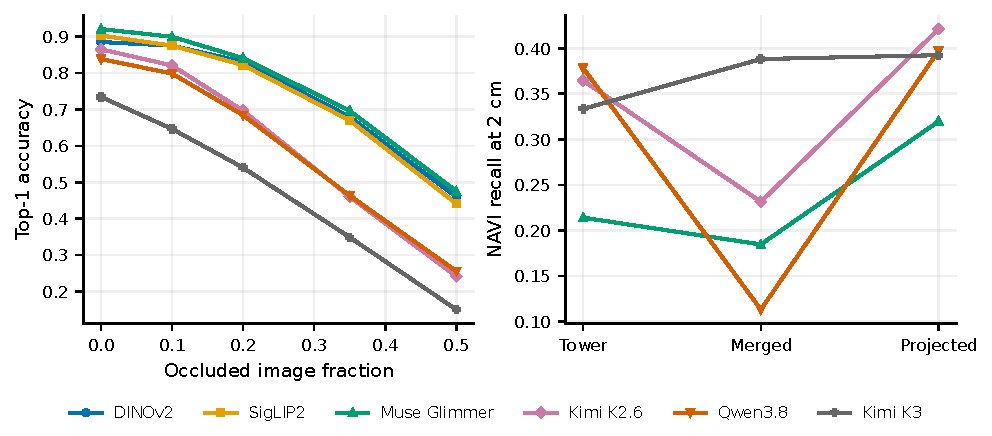
\includegraphics[width=0.9\textwidth]{figures/paper-secondary.pdf}
\caption{Left: absolute top-1 accuracy under occlusion at the tower stage, matched
attention readout. Right: training-free NAVI recall at the three native stages for
multimodal towers. Curves are descriptive; uncertainty is not plotted.}
\label{fig:secondary}
\end{figure}

\begin{table}[H]
\centering\small
\caption{Final-tower correspondence levels. SPair is a macro average over 18 classes;
its paired intervals above average over finite image pairs instead.}
\label{tab:correspondence}
\begin{tabular}{lrrr}
\toprule
Tower & NAVI & ScanNet & SPair (macro)\\
\midrule
DINOv2 & 0.5389 & 0.0896 & 0.5547\\
SigLIP2 & 0.4013 & 0.0584 & 0.3982\\
Muse Glimmer & 0.2139 & 0.0208 & 0.0909\\
Kimi K2.6 & 0.3646 & 0.0547 & 0.1782\\
Qwen3.8 & 0.3785 & 0.0834 & 0.3081\\
Kimi K3 & 0.3334 & 0.0258 & 0.2760\\
\bottomrule
\end{tabular}

\end{table}

\section{Result provenance and reproduction}
Source and results: \url{https://github.com/immanuel-peter/vision-tower-bench}.
Build instructions are in \texttt{paper/README.md}.
\texttt{paper/build\_assets.py} generates numerical assets from recorded JSONs, with input
hashes in \texttt{paper/asset-sources.json}.
\texttt{results/README.md} indexes the experiments and corrections.

\end{document}
